\documentclass[tikz,border=10pt]{standalone}

\begin{document}
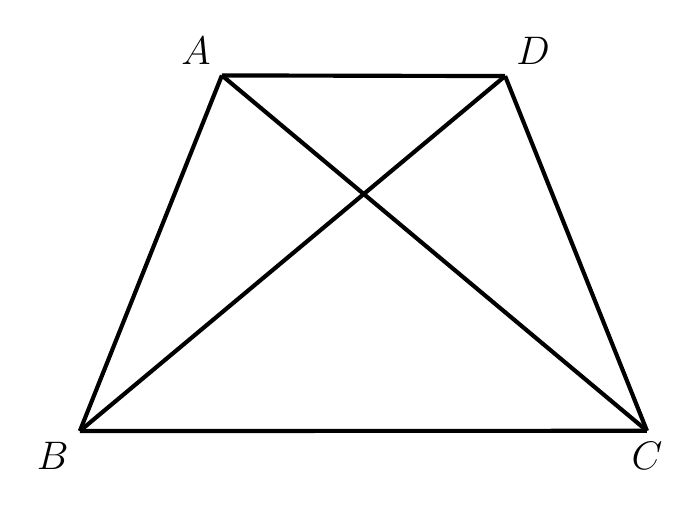
\begin{tikzpicture}[line width=1.5pt, line join=round]
\coordinate (A) at (-1.609,2.276);
\coordinate (B) at (-3.413,-2.240);
\coordinate (C) at (3.789,-2.237);
\coordinate (D) at (1.988,2.268);

  
  \draw (A) -- (B);
  \draw (B) -- (C);
  \draw (C) -- (D);
  \draw (D) -- (A);
  
  \draw (A) -- (C);
  \draw (B) -- (D);
  
  \node[above left,  font=\fontsize{15.5}{18.6}\selectfont] at (A) {$A$};
  \node[above right, font=\fontsize{15.5}{18.6}\selectfont] at (D) {$D$};
  \node[below left,  font=\fontsize{15.5}{18.6}\selectfont] at (B) {$B$};
  \node[below,       font=\fontsize{15.5}{18.6}\selectfont] at (C) {$C$};
\end{tikzpicture}
\end{document}